%-------------------------------------------------------------------------------------------------------
%-------------------------------------------------------------------------------------------------------
% Sec & Label

\section{Theoretical Analysis}
\label{sec:analysis}


%-------------------------------------------------------------------------------------------------------
%-------------------------------------------------------------------------------------------------------
% Intro

In this section, the Circuit T2 is analysed theoretically. In figure \ref{fig:Dsnh_oct_t2},
appart from all the components being identified, the assumed currents are also shown.
Only the node method was used in this section. Each subsection refers to each task.


Three important equations were used: both Kirchhoff's laws (Kirchhof's current law (KCL)
- eq.(\ref{eq:kcl}) and Kirchhoff's voltage law (KVL) - eq.(\ref{eq:kvl})); Ohm's law
(eq.(\ref{eq:ohm})).

The algebraic sum of all the currents in any given node is zero:
\begin{equation}
	\sum I_i = 0
	\label{eq:kcl}
\end{equation}

The algebraic sum of all the voltages in any given closed-loop circuit (mesh) is zero:
\begin{equation}
	\sum V_i = 0
	\label{eq:kvl}
\end{equation}

The potential difference between the two nodes connected to a resistor is equal to the current that 
passes through the resistor multiplied by its resistance.
\begin{equation}
	V_i = R_iI_i
	\label{eq:ohm}
\end{equation}

\begin{equation}
	V_1(t) = V_2(t) = V_2(\infty) + [V_2(0) - V_2(\infty)]e^{\frac{-t}{\tau}}
\end{equation}



%-----------------------------------------------------------------------
%-----------------------------------------------------------------------
% 			      task1 - subsec
% ----------------------------------------------------------------------
% ----------------------------------------------------------------------
\subsection{Task 1)}
\label{subsec:task1_a}

When $t<0$ the value of $V_s$ is constant and so we can perform DC analysis on the circuit. We can assume that enough time has passed and so it is reasonable to assume that the circuit is in steady-state.

When performing a DC steady-state analysis on a circuit we can use the fact that the current flowing trough the capacitor is null (the circuit behaves as if the capacitor was removed).

A node analysis was performed to find the voltage value of each node and the current in each branch.

The node method uses KCL in conjunction with Ohm’s law to define equations that when solved give the voltage value 
<<<<<<< HEAD
of each node in relation to ground (Node 0, $V_0 = 0$). In this circuit we defined six equations that equate the 
currents entering a particular node with the currents leaving said node. 
=======
of each nove in relation to ground (Node 4, $V_4 = 0$). 
>>>>>>> 406d41a171fa37743ffd3ada08d1bf50d815e525

In order to have equations that solve for the node’s voltage, a relation between curent and voltage is made using 
Ohm’s law (given a resistance between two nodes, the current that passes the resistance can be written as 
$I=\frac{V_2-V_1}{R_1}$)

To simplify the equations it is useful to use the conductance $G_n$ which is the inverse of the resistance $R_n$ 
($G_n=\frac{1}{R_n}$)

The equations used to solve the circuit were organized in matrix form.

{\footnotesize

$ \begin{bmatrix}
1 & 0 & 0 & 0 & 0 & 0 & 0 & 0 & 0 & 0 \\
G1 & -(G1+G2+G3) & G2 & G3 & 0 & 0 & 0 & 0 & 0 & 0 \\
0 & -G2 & G2 & 0 & 0 & 0 & 0 & 0 & -1 & 0 \\
0 & G3 & 0 & -(G3+G4+G5) & G5 & 0 & 0 & 0 & 0 & 0 \\
0 & 0 & 0 & -G5 & G5 & 0 & 0 & 0 & 1 & 1 \\
0 & 0 & 0 & 0 & 0 & G7 & -G7 & -1 & 0 & 1 \\
0 & 0 & 0 & 0 & 0 & -(G6+G7) & G7 & 0 & 0 & 0 \\
0 & 0 & 0 & 0 & 0 & 0 & 0 & 0 & 0 & 1 \\
0 & 0 & 0 & 1 & 0 & G6*K_d & -1 & 0 & 0 & 0 \\
0 & K_b & 0 & -K_b & 0 & 0 & 0 & 0 & -1 & 0 
\end{bmatrix}  $
$ \begin{bmatrix}
V1 \\
V2 \\
V3 \\
V5 \\
V6 \\
V7 \\
V8 \\
IH1 \\
Ib \\
Ic \\
\end{bmatrix}  $
=
$ \begin{bmatrix}
Vs\\
0\\
0\\
0\\
0\\
0\\
0\\
0\\
0\\
0\\
\end{bmatrix}  $
}

Figure \ref{fig:Desenho_t2}. In adition, assume $V_{Ni}$ to be the voltage in node $Ni$ (every node position can
also be found in Figure \ref{fig:Desenho_t2}). \\

\begin{figure}[ht]
	\centering
	\includegraphics[width=0.75\linewidth]{dsnh_oct_t2_al1.pdf}
	\caption{Circuit T2, analysed by Ngspice}
\label{fig:Dsnh_sim_t2}
\end{figure}






{\footnotesize

$ \begin{bmatrix}
1 & 0 & 0 & 0 & 0 & 0 & 0 & 0 & 0 & 0 \\
G1 & -(G1+G2+G3) & G2 & G3 & 0 & 0 & 0 & 0 & 0 & 0 \\
0 & -G2 & G2 & 0 & 0 & 0 & 0 & 0 & -1 & 0 \\
0 & G3 & 0 & -(G3+G4+G5) & G5 & 0 & 0 & 0 & 0 & 0 \\
0 & 0 & 0 & -G5 & G5 & 0 & 0 & 0 & 1 & 1 \\
0 & 0 & 0 & 0 & 0 & G7 & -G7 & -1 & 0 & 1 \\
0 & 0 & 0 & 0 & 0 & -(G6+G7) & G7 & 0 & 0 & 0 \\
0 & 0 & 0 & 0 & 0 & 0 & 0 & 0 & 0 & 1 \\
0 & 0 & 0 & 1 & 0 & G6*K_d & -1 & 0 & 0 & 0 \\
0 & K_b & 0 & -K_b & 0 & 0 & 0 & 0 & -1 & 0 
\end{bmatrix}  $
$ \begin{bmatrix}
V1 \\
V2 \\
V3 \\
V5 \\
V6 \\
V7 \\
V8 \\
IH1 \\
Ib \\
Ic \\
\end{bmatrix}  $
=
$ \begin{bmatrix}
V1 \\
V2 \\
V3 \\
V5 \\
V6 \\
V7 \\
V8 \\
IH1 \\
Ib \\
Ic \\
\end{bmatrix}  $
}

{\footnotesize

$ \begin{bmatrix}
1 & 0 & 0 & 0 & 0 & 0 & 0 & 0 & 0 & 0 \\
G1 & -(G1+G2+G3) & G2 & G3 & 0 & 0 & 0 & 0 & 0 & 0 \\
0 & -G2 & G2 & 0 & 0 & 0 & 0 & 0 & -1 & 0 \\
0 & G3 & 0 & -(G3+G4+G5) & G5 & 0 & 0 & 0 & 0 & 0 \\
0 & 0 & 0 & -G5 & G5 & 0 & 0 & 0 & 1 & 1 \\
0 & 0 & 0 & 0 & 0 & G7 & -G7 & -1 & 0 & 1 \\
0 & 0 & 0 & 0 & 0 & -(G6+G7) & G7 & 0 & 0 & 0 \\
0 & 0 & 0 & 0 & 1 & 0 & -1 & 0 & 0 & 0 \\
0 & 0 & 0 & 1 & 0 & G6*K_d & -1 & 0 & 0 & 0 \\
0 & Kb & 0 & -K_b & 0 & 0 & 0 & 0 & -1 & 0 
\end{bmatrix}  $
$ \begin{bmatrix}
V1 \\
V2 \\
V3 \\
V5 \\
V6 \\
V7 \\
V8 \\
IH1_2 \\
Ib_2 \\
Ic_2 \\
\end{bmatrix}  $
=
$ \begin{bmatrix}
V1 \\
V2 \\
V3 \\
V5 \\
V6 \\
V7 \\
V8 \\
IH1 \\
Ib \\
Ic \\
\end{bmatrix}  $

$ \begin{bmatrix}
1 & 0 & 0 & 0 & 0 & 0 & 0 & 0 & 0 & 0 \\
G1 & -(G1+G2+G3) & G2 & G3 & 0 & 0 & 0 & 0 & 0 & 0 \\
0 & -G2 & G2 & 0 & 0 & 0 & 0 & 0 & -1 & 0 \\
0 & G3 & 0 & -(G3+G4+G5) & G5 & 0 & 0 & 0 & 0 & 0 \\
0 & 0 & 0 & -G5 & G5 & 0 & 0 & 0 & 1 & 1 \\
0 & 0 & 0 & 0 & 0 & G7 & -G7 & -1 & 0 & 1 \\
0 & 0 & 0 & 0 & 0 & -(G6+G7) & G7 & 0 & 0 & 0 \\
0 & 0 & 0 & 0 & -1/Z_c & 0 & 1/Z_c & 0 & 0 & 0 \\
0 & 0 & 0 & 1 & 0 & G6*K_d & -1 & 0 & 0 & 0 \\
0 & K_b & 0 & -K_b & 0 & 0 & 0 & 0 & -1 & 0 
\end{bmatrix}  $
$ \begin{bmatrix}
V1_3 \\
V2_3 \\
V3_3 \\
V5_3 \\
V6_3 \\
V7_3 \\
V8_3 \\
\end{bmatrix}  $
=
$ \begin{bmatrix}
V1 \\
V2 \\
V3 \\
V5 \\
V6 \\
V7 \\
V8 \\
IH1 \\
Ib \\
Ic \\
\end{bmatrix}  $
}

With these 8 equations it is possible to solve the system using Octave.
The results were organized in Table \ref{tab:node}

\begin{table}[ht]
	\centering
	\begin{tabular}{|l|r|}
    		\hline    
    		{\bf Name} & {\bf Value [A or V]} \\ \hline
    		$V_{N1}$ & 5.114025e+00 \\ \hline 
$V_{N2}$ & 4.830792e+00 \\ \hline 
$V_{N3}$ & 4.226624e+00 \\ \hline 
$V_{N5}$ & 4.871651e+00 \\ \hline 
$V_{N6}$ & 5.781844e+00 \\ \hline 
$V_{N7}$ & -1.849204e+00 \\ \hline 
$V_{N8}$ & -2.786253e+00 \\ \hline 
$@I_{b}$ & -2.957272e-04 \\ \hline 
$@I_{c}$ & 0.000000e+00 \\ \hline 
$@I_{R1}$ & 2.822201e-04 \\ \hline 
$@I_{R2}$ & -2.957272e-04 \\ \hline 
$@I_{R3}$ & -1.350709e-05 \\ \hline 
$@I_{R4}$ & 1.200956e-03 \\ \hline 
$@I_{R5}$ & -2.957272e-04 \\ \hline 
$@I_{d}$ & -9.187358e-04 \\ \hline 
$@I_{R6}$ & 9.187358e-04 \\ \hline 

  	\end{tabular}
  	\caption{Values computed by Octave. Variables identified with a '$@$' have a
  	corresponding value in Ampere (A). The others are expressed in Volts (V).}
 
\label{tab:node}
\end{table}

%-----------------------------------------------------------------------
%-----------------------------------------------------------------------
% 			      task2 - subsec
% ----------------------------------------------------------------------
% ----------------------------------------------------------------------
\subsection{Task 2)}
\label{subsec:task2_a}

\begin{figure}[ht]
	\centering
	\includegraphics[width=0.75\linewidth]{dsnh_oct_t2_al2.pdf}
	\caption{Circuit T2, analysed by Ngspice}
\label{fig:Dsnh_sim_t2}
\end{figure}

%-----------------------------------------------------------------------
%-----------------------------------------------------------------------
% 			      task3 - subsec
% ----------------------------------------------------------------------
% ----------------------------------------------------------------------
\subsection{Task 3)}
\label{subsec:task3_a}

\begin{figure}[ht]
	\centering
	\includegraphics[width=0.75\linewidth]{dsnh_oct_t2_al3.pdf}
	\caption{Circuit T2, analysed by Ngspice}
\label{fig:Dsnh_sim_t2}
\end{figure}

\begin{figure}[ht]
	\centering
	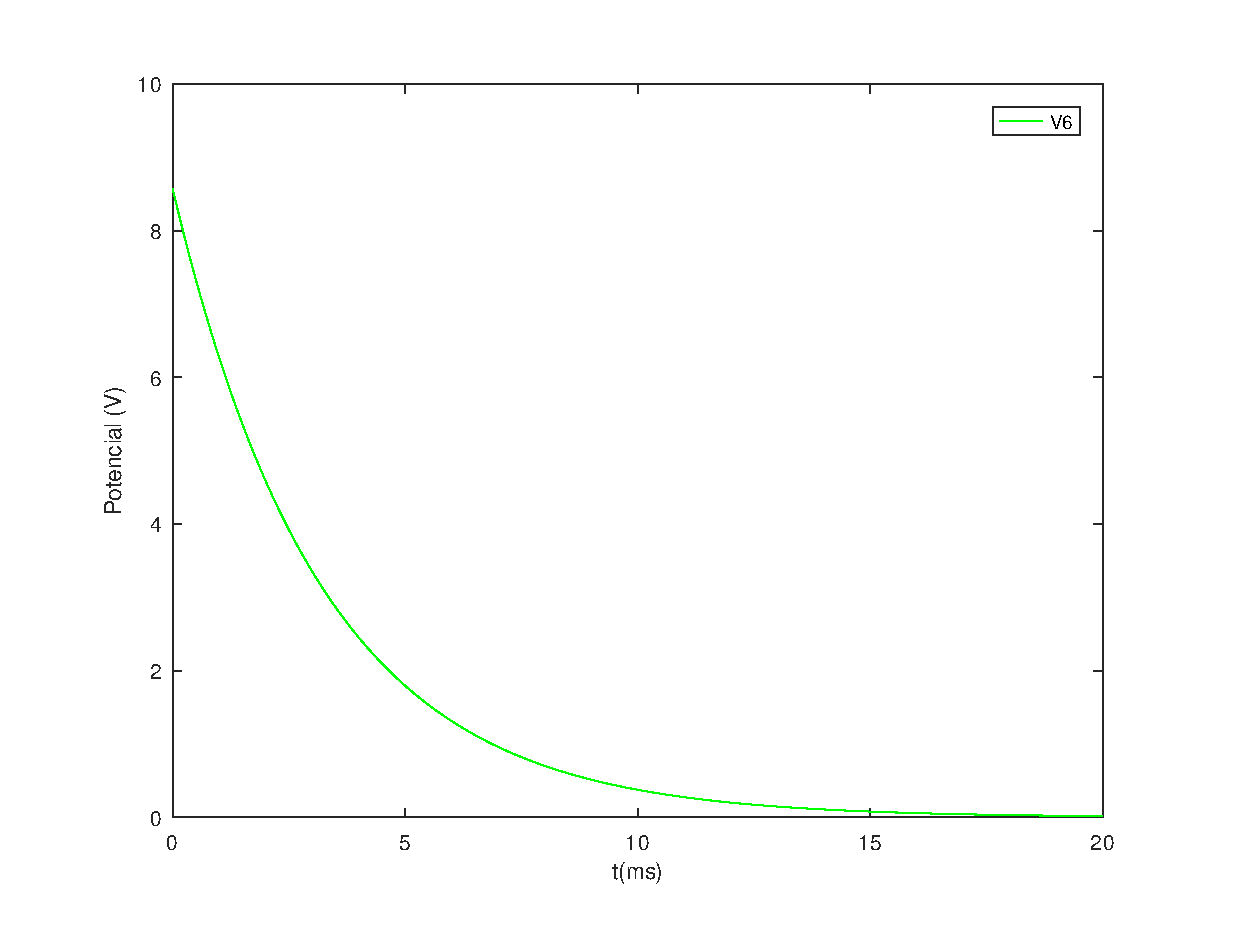
\includegraphics[width=0.55\linewidth]{plot1.eps}
	\caption{Plot oct - 1}
\label{fig:Dsnh_sim_t2}
\end{figure}

%-----------------------------------------------------------------------
%-----------------------------------------------------------------------
% 			      task4 - subsec
% ----------------------------------------------------------------------
% ----------------------------------------------------------------------
\subsection{Task 4)}
\label{subsec:task4_a}

\begin{figure}[ht]
	\centering
	\includegraphics[width=0.75\linewidth]{dsnh_oct_t2_al456.pdf}
	\caption{Circuit T2, analysed by Ngspice}
\label{fig:Dsnh_sim_t2}
\end{figure}

%-----------------------------------------------------------------------
%-----------------------------------------------------------------------
% 			      task5 - subsec
% ----------------------------------------------------------------------
% ----------------------------------------------------------------------
\subsection{Task 5)}
\label{subsec:task5_a}


\begin{figure}[ht]
	\centering
	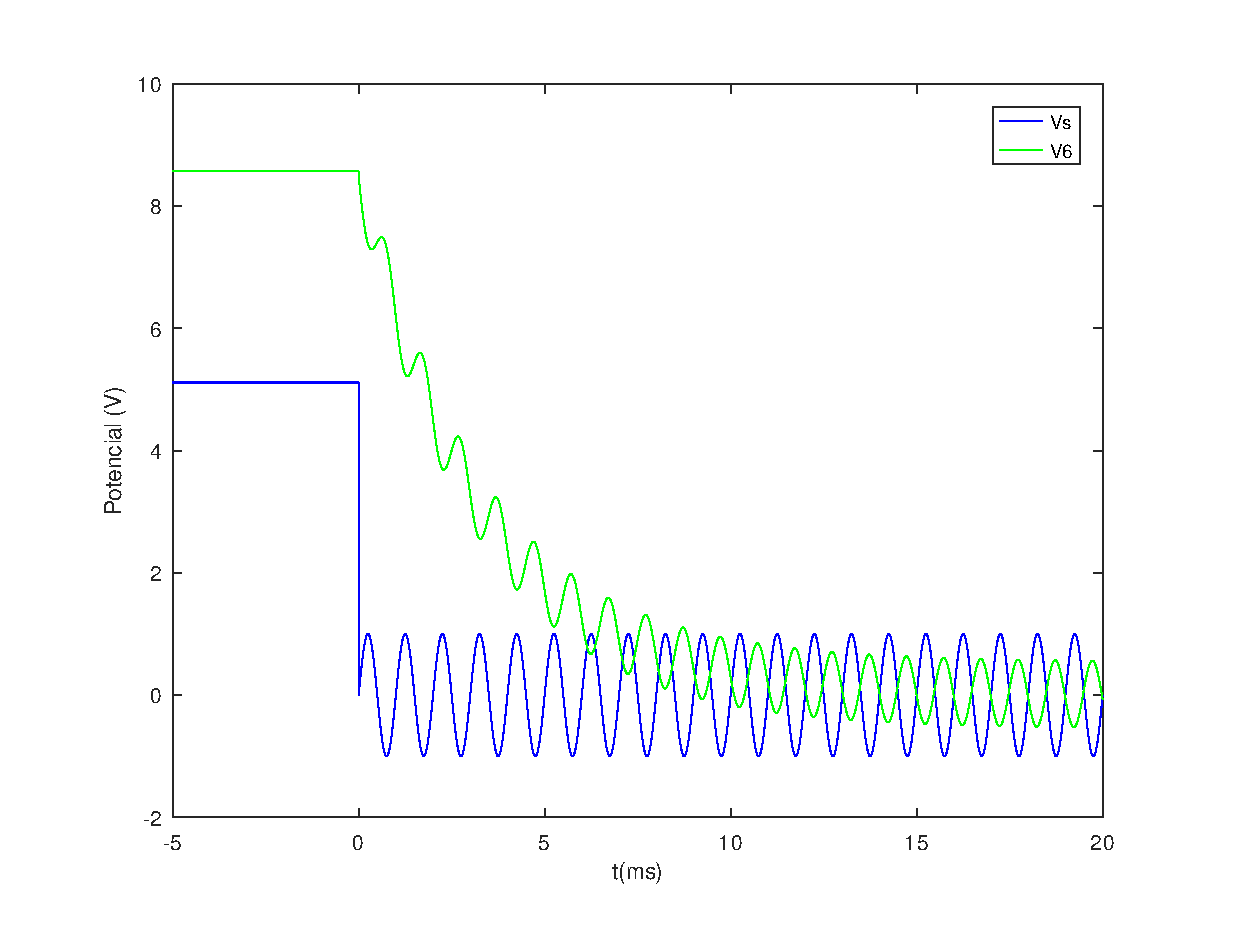
\includegraphics[width=0.55\linewidth]{plot2.eps}
	\caption{Plot oct - 2}
\label{fig:Dsnh_sim_t2}
\end{figure}

%-----------------------------------------------------------------------
%-----------------------------------------------------------------------
% 			      task6 - subsec
% ----------------------------------------------------------------------
% ----------------------------------------------------------------------
\subsection{Task 6)}
\label{subsec:task6_a}

\begin{figure}[ht]
	\centering
	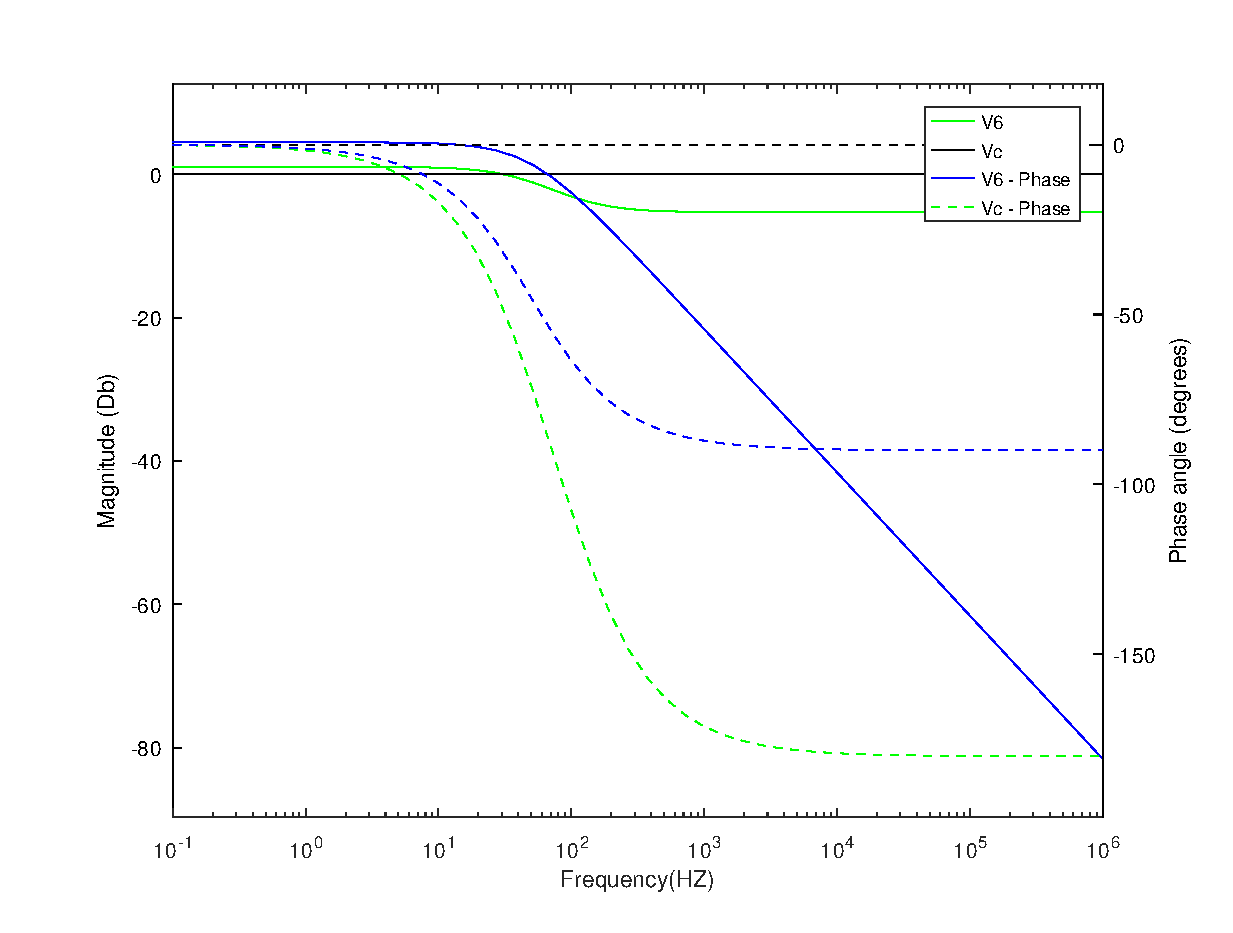
\includegraphics[width=0.55\linewidth]{plot3.eps}
	\caption{Plot oct - 3}
\label{fig:Dsnh_sim_t2}
\end{figure}



